% !TeX encoding = UTF-8
% !TeX spellcheck = de_DE
% !TeX root = ./mainDoc.tex

\section{JavaScript Grundlagen}

Bevor die JavaScript Spezifika der Code-Wiederverwendung besprochen werden können, müssen einige Besonderheiten der Programmiersprache und des damit einhergehenden Programmierparadigmas besprochen werden.

JavaScript ist eine objektorientierte (OO) Programmiersprache, die jedoch im Gegensatz zur großen Mehrzahl anderer Sprachen nicht \emph{klassenbasiert} sondern \emph{prototypenbasiert} ist. Neben dem objektorientierten Paradigma kann JavaScript auch als funktionale Programmiersprache aufgefasst werden, da Funktionen in JavaScript \emph{normale} Objekte, und damit "`1st-class values"' sind. Sie können wie jedes andere Objekt an Variablen gebunden werden und damit sowohl als Parameter als auch als Rückgabewerte von Funktionsaufrufen verwendet werden. 

Auf diese beiden Eigenschaften und die daraus resultierenden Konsequenzen für die Wiederverwendung von Code soll im folgenden einleitenden Abschnitt kurz eingegangen werden.

\subsection{Prototypische Objektorientierung}

Die meisten landläufig bekannten OO-Programmiersprachen basieren auf Klassen\footnote{Eine Übersicht kann hier der Wikipedia Eintrag \url{https://en.wikipedia.org/wiki/List_of_programming_languages_by_type\%23Object-oriented_class-based_languages} liefern.}. Dazu gehört auch die an der FernUni Hagen als Standard-OO-Sprache gelehrte Sprache Java.

%Klassisch: 
%- In klassischen OO-Sprachen wird zunächst eine Klasse als Blaupause definiert. 
%- Ein konkretes Objekt wird erzeugt indem eine "`Kopie"' dieser Blaupause materialisiert wird.
%- Es gibt kein Objekt ohne vorherige Klassendefinition.

In diesen klassischen OO-Sprachen wird zunächst eine Klasse definiert, die als Blaupause, bzw. abstraktes Modell für Objekte eines bestimmten Typs dient. Wenn die Programmiererin ein konkretes Objekt --eine Instanz-- benötigt, so wird es anhand dieses vorher definierten Bauplans erstellt. Es handelt sich damit um die "`materialisierte Kopie"' des Bauplans. In der klassischen Objektorientierung gibt es kein Objekt, zu dem nicht im Vorfeld eine Klasse definiert wurde (siehe \citep[p. 69]{SimpsonThisobjectprototypes2014}).

%\skippingparagraph

%JS: 
%- Objekte stehen für sich und werden einzeln erzeugt. Jedes Objekt hat einen Prototyp, der auch von mehreren Objekten gemeinsam verwendet werden kann, so dass gemeinsame Objekteigenschaften dort gebündelt werden können.
%- Obwohl in JS seit Version ES6 das Schlüsselwort \texttt{class} eingeführt wurde, handelt es sich nicht um einen echten Klassenmechanismus, wie man ihn von klassische Sprachen her kennt. Das Prototyp-Paradigma gibt es jedoch her, dass ein Klassenmechanismus nachgebildet werden kann.
%- Objekt kann Properties enthalten
%	- Diese sind entweder ein primitiver Typ
%	- Oder eine Referenz auf ein Objekt

Im Gegensatz dazu stehen Objekte in prototypbasierten Sprachen für sich allein. Sie können "`out of thin air"' (\citep[p. 21]{SimpsonThisobjectprototypes2014}) erzeugt werden, ohne dass vorher ein Modell des Objekts definiert werden muss. 

%Ein solches Objekt kann über eine interne Verknüpfung mit einem bereits bestehenden Objekt verbunden werden und so dessen Eigenschaften und Verhalten per Delegation nutzen. Es \emph{erbt} damit die Eigenschaften des verknüpften Objekts. Da der Link zu einem anderen Objekt in der ECMAScript Spezifikation (\citep{international2018ecmascript}) als [[Prototype]]-Link bezeichnet wird, spricht man auch davon, dass ein Objekt der \emph{Prototyp} für ein anderes Objekt ist.

Ein Objekt in JavaScript selber ist eine Sammlung von benannten \emph{Properties}, denen Werte zugeordnet werden können. Die Struktur ist damit vergleichbar mit einer \emph{Dictionary}-Datenstruktur aus \texttt{\{key: value\}} mit dem Property-Namen als \texttt{key}. Diesem Dictonary, und damit dem Objekt, können zur Laufzeit weitere Properties hinzugefügt oder auch wieder daraus gelöscht werden.

Die Werte der Properties sind entweder \emph{Referenzen} auf ein weiteres Objekt oder ein \emph{primitiver Wert}. Als primitive Werte sind in JavaScript lediglich die Typen \texttt{Undefined}, \texttt{Null}, \texttt{Boolean}, \texttt{Number}, \texttt{Symbol}, und \texttt{String} definiert (siehe \citep[§4.3.2]{international2018ecmascript}). Alle anderen Werte, und insbesondere Funktionen, sind selber Objekte, auf die eine Property referenzieren kann. Bei Funktionen, die einer Objekt-Property zugeordnet sind, spricht man von \emph{Methoden}.


%\todo{Wo kommt dynamisch vs. feste Objekte rein?}

\subsection{Die Prototype-Chain}

%Klassisch:
%- In der Definition einer klasse wird eine Parent-Klasse angegeben
%- Child-Klassen erben alle Eigenschaften der Parent-Klasse
%- Sie können weitere Properties und Methoden dazu definieren
%- Sie können Properties und Methoden der Parent-Klasse überschreiben und damit verändern
%- Der Zugriff auf die Methoden und Properties der Parent-Klasse ist üblicherweise über \texttt{super} möglich



%\skippingparagraph

%JS:
%- jedes Objekt hat eine Referenz auf [[Prototype]]
%- [[Prototype]] kann \texttt{null} sein (z. B. bei \texttt{Object} der Fall, das ganz oben in der Vererbungshierarchie steht)
%- [[Prototype]] ist ein normales Objekt und kann Properties und Methoden enthalten
%- [[Prototype]] hat selber wieder eine Referenz auf einen [[Prototype]], bis die Referenz auf \texttt{null} zeigt
%- Es bildet sich eine Prototype-Chain
%- Alles in [[Prototype]] wird von den Objekten, deren Referenz auf das gleiche Objekt zeigt gemeinsam genutzt
%- Damit lässt sich auch in JS eine Vererbungshierarchie aufbauen
%- Scoping und Prototype-Chain:
%- Bei Zugriff auf eine Property eines Objekts wird zunächst nach einer eigenen Property gesucht
%- Falls keine Property gefunden wird, wird im [[Prototype]] nachgesehen, dann im [[Prototype]]  von [[Prototype]], usw.
%- Sobald eine passende Property gefunen wird, so wird diese benutzt
%- Shadowing
%- Properties mit gleichen Namen verdecken [[Prototype]]-Properties weiter oben in der Hierarchie
%- kann manchmal zu ungewollten Effekten führen, insbesondere, wenn 
%- falsch auf Properties zugegriffen wird, die dann im Objekt angelegt werden
%- wenn die Properties Referenzen sind, dann ist shadowing wieder etwas anders

%Durch den [[Prototype]]-Mechanismus lässt sich eine Vererbungshierarchie aufbauen wie in klassischen Sprachen. Lediglich der einfache Zugriff auf \texttt{super} funktioniert nicht. (Das ist in \texttt{class} zwar nachgebildet, wird hier nicht weiter besprochen.) Daher sollte man keine Methoden überschreiben, die Zugriff auf übergeordnete Funktion gleichen Namens braucht. Dafür gibt es Techniken.


%In JavaScript ist es möglich Objekthierarchien aufzubauen.
%%gibt es keine Klassen, sondern lediglich einzelne Objekte. Trotzdem ist es auch in JavaScript möglich Objekthierarchien aufzubauen, in denen die Eigenschaften eines allgemeineren (Eltern-)Objekts an davon abgeleitete (Kind-)Objekte weitergegeben werden. 
%Zur Realisierung solcher Objekthierarchien besitzt in Javascript jedes Objekt einen sogenannten \emph{[[Prototype]]}-Slot, dessen Wert entweder \texttt{Null} oder eine Referenz auf ein Objekt ist. Über die in [[Prototype]] enthaltene Referenz kann ein Objekt an das damit verlinkte Objekt delegieren. So sind die Properties des verlinkten Objekts vom Verlinkenden aus sichtbar (siehe \citep[§9.1]{international2018ecmascript}). 
%%Seit ES6 ist der [[Prototype]]-Slot eines Objekts direkt über die Property \texttt{.\_\_protot\_\_} eines Objekts zugreifbar.
%
%\begin{figure}[h]
%	\centering
%	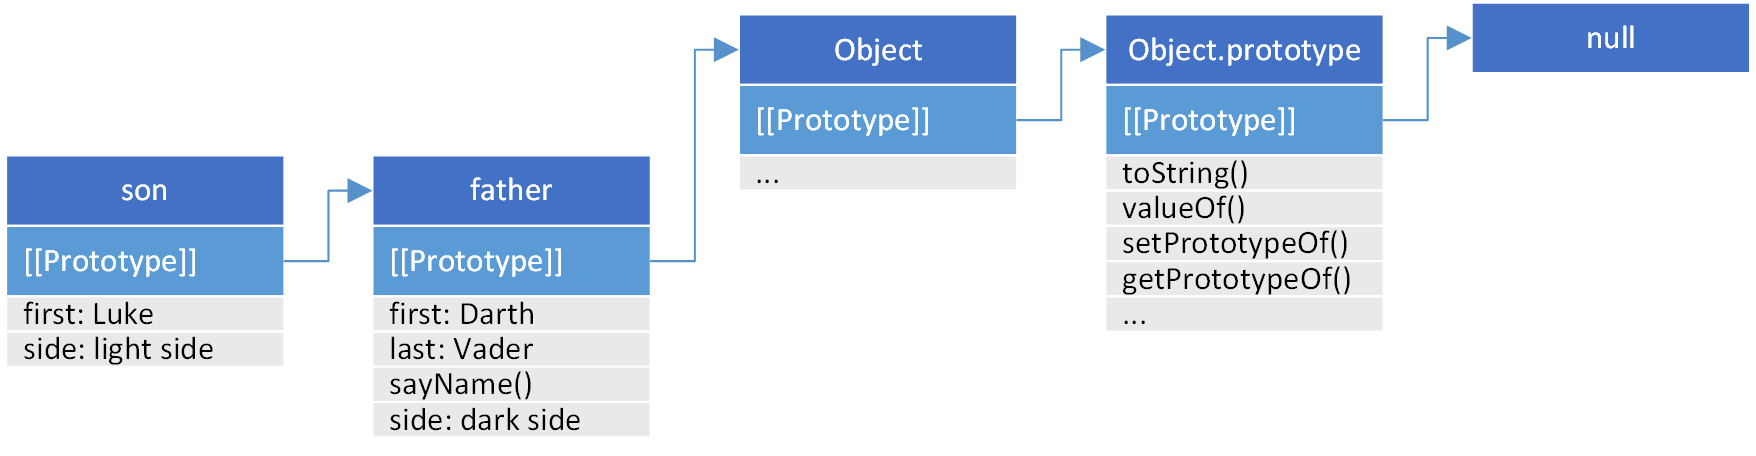
\includegraphics[width=0.8\textwidth]{images/prototypeChain.png}
%	\caption{\label{prototypeChain}Dlegeations-Links entlalang der Prorotype-Chain (aus \citep[p. 118]{StefanovJavaScriptpatternsbuild2010}}
%\end{figure}
%
%
%Wenn in JavaScript auf die Property eines Objekts, sei es ein primitiver Wert oder eine Objektreferenz, zugegriffen wird, so wird zunächst überprüft ob das Objekt eine eigene Property des gewünschten Namens besitzt. Ist dies der Fall, so erfolgt der Zugriff darauf. Ist keine eigene Property des gewünschten Namens vorhanden, so wird im [[Prototype]] des Objekts nachgesehen, ob die gesuchte Property dort vorhanden ist.
%Da auch das [[Prototype]]-Objekt selber ein Objekt ist enthält es auch selber eine Referenz auf ein weiteres [[Prototype]]-Objekt, das in der Hierarchie weiter oben steht. Es entsteht die sogenannte \emph{Prototype-Chain}, entlang derer JavaScript nach einer gewünschten Property sucht, bis diese entweder gefunden wird, oder aber das oberste Objekt der Prototype-Chain als eigenen [[Prototype]] einen Verweis auf \texttt{null} besitzt und die Kette damit am Ende ist. Erst wenn entlang dieser Kette die gewünschte Property nicht gefunden wird, stellt die JavaScript Laufzeitumgebung fest, dass eine Property nicht vorhanden ist und gibt \texttt{undefined} zurück.
%
%Mittels dieses Mechanismus von JavaScript lässt sich auf natürliche Weise eine Delegationshierarchie aufbauen: Gemeinsam genutzte Properties und Methoden werden in einem Objekt definiert, das in den Kind-Objekten, die diese nutzen wollen, als [[Prototype]] referenziert wird. Dadurch können alle Kind-Objekte die auf dem [[Prototype]] definierten Properties und Methoden benutzen. Wenn in einem Objekt für eine Property ein verändertes Verhalten erwünscht ist, so kann einfach eine eigene Property gleichen Namens angelegt werden, welche die ansonsten gemeinsam genutzte Property verdeckt (\emph{shadowing}) und damit deren Verhalten überschreibt.
%
%Änderungen des [[Prototype]] haben Auswirkungen auf alle darauf referenzierenden Objekte, es sei denn die geänderte Property wird weiter unten in der Hierarchie durch eine eigene Property verdeckt. Daher ist bei der Zuweisung von Werten darauf zu achten, ob man gerade auf eine eigene Property zugreift oder auf eine in der Prototype-Chain weiter oben liegende. 
%%Dies kann mittels der Funktion \texttt{Object.prototype.hasOwnProperty()} überprüft werden. 
%
%Wenn es darauf ankommt zu wissen, ob ein Objekt eine Property selber besitzt, oder per Delegation entlang der Prototype-Chain darauf zugreift, so kann dies über die Methode \texttt{obj.hasOwnProperty(prop)} geprüft werden. Diese ist definiert als \texttt{Object.proto\-type.hasOwnProperty()} und wird daher auf einem Objekt \texttt{obj} per Delegation an \texttt{Object.prototype} aufgerufen. Seit der Version ES6  können die eigenen Properties eines Objekts über die funktion \texttt{Object.keys(obj)} als Array abgefragt werden.\footnote{Genau genommen beziehen sich die beiden genannten Funktionen lediglich auf Objektproperties, die als \texttt{enumerable: true} gekennzeichnet sind.}


JavaScript hat einen eingebauten Delegationsmechanismus bezüglich des Zugriffs auf Objekt-Properties. Dazu hat jedes Objekt eine interne Referenz --in der Sprachspezifikation \citep[§9.1]{international2018ecmascript} als \emph{[[Prototype]]}"~Slot bezeichnet-- die entweder auf ein anderes Objekt zeigt oder den primitiven Wert \texttt{null} enthält. Das referenzierte Objekt wird \emph{Prototyp} genannt. Da ein so referenziertes Objekt selber wieder eine Referenz auf einen eigenen Prototypen enthält, ergibt sich eine verkette Liste aus Objekt-Referenzen, die als \emph{Prototype-Chain} bezeichnet wird. 
In der Regel endet die Prototype-Chain im Objekt \texttt{Object.prototype}, auf dem einige nützliche Hilfsfunktionen (z.~B. \texttt{toString() oder \texttt{valueOf()}}) als Properties implementiert sind.

Der Prototyp eines Objekts wird automatisch bei der Objekterzeugung gesetzt und kann über \texttt{Object.getPrototypeOf()} abgefragt bzw. über \texttt{Object.setPrototypeOf()} geändert werden. 
Wie die automatische Setzung erfolgt, wird später im Abschnitt zur Objekterzeugung detailliert erläutert.

Bei einem lesenden Zugriff oder einem Funktionsaufruf auf eine Objekt-Property wird zunächst durch die Runtime geprüft, ob das Objekt selber eine Property entsprechenden Namens hat. Ist dies nicht der Fall, so folgt die Runtime der [[Prototype]]-Referenz und sucht im Prototyp-Objekt nach der passenden Property. Wenn diese dort gefunden wird, so erfolgt der Zugriff darauf. Andernfalls wird die Suche nach der Property entlang der Prototype-Chain fortgesetzt, bis sie entweder gefunden wird, oder die Kette endet. Dieser automatische Zugriff auf Properties von Objekten, die in der Prototypen-Hierarchie weiter oben stehen, entspricht einer Delegation an ein anderes Objekt und umfasst insbesondere auch Methodenaufrufe.

Diese automatische Delegation erfolgt nur bei lesenden Zugriffen auf Properties. Da schreibende Zugriffe auf eine Property Auswirkungen auf alle, in der Prototype-Chain tiefer liegenden Objekte haben, werden Änderungen per Delegation von einem tiefer liegenden Objekt aus verhindert. Bei einem schreibenden Zugriff auf eine Property, die weiter oben in der Prototype-Chain definiert und nicht als \emph{read-only} markiert ist, wird auf dem Startobjekt der Prototype-Chain eine neue Property des gleichen Namens angelegt. Diese neue Property verdeckt bei darauffolgenden lesenden Zugriffen die weiter oben liegende Property des Prototypen. Man spricht in diesem Fall von \emph{shadowing}.\footnote{Der Vollständigkeit halber sei erwähnt, dass eine weiter oben in der Chain liegende Property in Ausnahmefällen verändert werden kann, wenn diese nicht als normale Property, sondern über einen \emph{Setter} definiert ist. Dies ist in der Praxis jedoch die Ausnahme und wird daher hier nicht weiter ausgeführt. Details finden sich in \citep[p. 88f.]{SimpsonThisobjectprototypes2014} und in \citep{international2018ecmascript}.}

Änderungen direkt am Prototypen-Objekt dagegen haben Auswirkungen auf alle darauf referenzierenden Objekte, es sei denn, die geänderte Property wird weiter unten in der Hierarchie verdeckt. Daher ist bei der Zuweisung von Werten darauf zu achten, ob man gerade auf eine eigene Property zugreift oder auf eine in der Prototype-Chain weiter oben liegende. 
Wenn es darauf ankommt zu wissen, ob ein Objekt eine Property selber besitzt, oder per Delegation entlang der Prototype-Chain darauf zugreift, so kann dies über die Methode \texttt{obj.hasOwnProperty(prop)} geprüft werden. Diese ist definiert als \texttt{Object.proto\-type.hasOwnProperty()} und wird daher auf einem Objekt \texttt{obj} per Delegation an \texttt{Object.prototype} aufgerufen. Seit der Version ES6  können die eigenen Properties eines Objekts über die Funktion \texttt{Object.keys(obj)} direkt als Array abgefragt werden (siehe \citep[§19.1.2.16]{international2018ecmascript}).%\footnote{Genau genommen beziehen sich die beiden genannten Funktionen lediglich auf Objektproperties, die als \texttt{enumerable: true} gekennzeichnet sind.}

\skippingparagraph

\insertcode{codesnips/prototypeChain.js}{Beispiel von Delegation und Shadowing in der Prototype Chain}

Zur Verdeutlichung sei hier ein kleines Beispiel angegeben. In Listing \ref{codesnips/prototypeChain.js} wird ein \texttt{father} und ein \texttt{son}-Objekt erstellt. Die [[Prototype]]-Referenz von \texttt{son} wird explizit auf \texttt{father} gesetzt und hat damit per Delegation Zugriff auf dessen Properties inklusive der Methode \texttt{sayName()}. 

Zunächst hat \texttt{son} keine eigenen Properties, kann aber per Delegation auf die Properties von \texttt{father} zugreifen. Die Zuweisung in Zeile 14 erzeugt eine neue Property \texttt{first} auf dem Objekt \texttt{son}, welche die gleichnamige Property von \texttt{father} überdeckt. In Zeile 20 wird \texttt{father.name} geändert. Das hat auch (häufig ungewollte) Auswirkungen auf den Property-Lookup des \texttt{son}-Objekts aus. In den Zeilen 24-31 sind weitere Ausgaben zu sehen, die das Verhalten verdeutlichen. In Abbildung \ref{prototypeChain} ist die Prototype-Chain ausgehend von \texttt{son} zum Programmende schematisch dargestellt.

\begin{figure}[h]
	\centering
	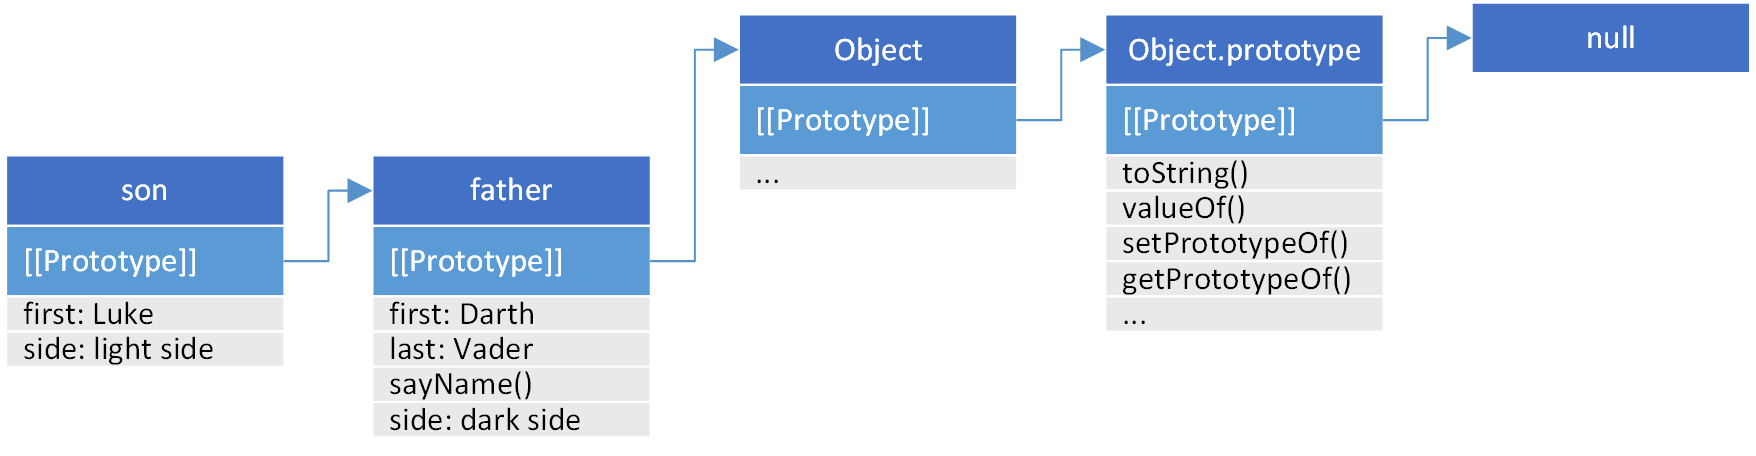
\includegraphics[width=1\textwidth]{images/prototypeChain.png}
	\caption{\label{prototypeChain}Die Prototype-Chain der Objekte aus Listing \ref{codesnips/prototypeChain.js}.}
\end{figure}



%Mittels der beschriebenen Mechanismen von JavaScript lässt sich auf natürliche Weise eine Delegationshierarchie aufbauen: Gemeinsam genutzte Properties und Methoden werden in einem Prototyp-Objekt definiert, und können von darauf verweisenden Kind-Objekten benutzt werden. Wenn in einem Objekt für eine Property ein verändertes Verhalten erwünscht ist, so kann einfach eine eigene Property gleichen Namens angelegt werden, welche die ansonsten gemeinsam genutzte Property verdeckt (\emph{shadowing}) und damit deren Verhalten überschreibt.


\subsection{\texttt{this}-Binding}

%JS:
%In Js ist das \texttt{this}-Binding etwas speziell und daher mit Vorsicht zu genießen:
%- \texttt{this}-Binding ist etwas speziell und kann sich auf verschiedene Dinge beziehen
%	- 4 Varianten aus Kyle

In OO-Sprachen wird eine Möglichkeit benötigt, mit der eine Methode eines Objekts auf die Properties eben dieses Objekts zugreifen kann. In den meisten OO-Pro\-gram\-mier\-spra\-chen gibt es dazu das Schlüsselwort \texttt{this}\footnote{
Der Name des Schlüsselworts variiert in verschiedenen Sprachen.
}, welches an die gerade aktuelle Objektinstanz gebunden ist. 

Auch JavaScript hat das Schlüsselwort \texttt{this} definiert, welches bei einem Funktionsaufruf zur Laufzeit an ein Objekt gebunden wird. An welches Objekt \texttt{this} gebunden wird, ist davon abhängig wie die Funktion aufgerufen wird. Die konkrete Bindung zur Laufzeit gibt den Kontext vor, in dem die Funktion ausgeführt wird und auf dessen Properties sie Zugriff hat. 

Es gibt im Wesentlichen vier Regeln, nach denen die Laufzeitumgebung entscheidet, auf welches Objekt \texttt{this} referenziert. Diese Regeln werden der Reihe nach geprüft und die zuerst zutreffende Regel wird verwendet, um die passende Referenz in \texttt{this} abzulegen:
\begin{enumerate}
	\item \emph{new binding}
	\item \emph{explicit binding}
	\item \emph{implicit binding}
	\item \emph{default binding}
\end{enumerate}

Zusätzlich gibt es seit der Sprachversion ES6 noch einen Bindungsmechanismus, welcher die aufgezählten Regeln außer Kraft setzt:
ES6 \emph{arrow functions} benutzen einen \emph{lexikalischen Kontext} (\emph{lexical scope}) und damit eine feste \texttt{this}-Bindung, die nicht erst zur Laufzeit erstellt wird.

\paragraph{new binding} Wenn eine Funktion als Konstruktorfunktion mit dem Schlüsselwort \texttt{new} aufgerufen wird, so erzeugt sie ein neues Objekt (siehe unten \ref{Objekterzeugung}). Innerhalb der Konstruktorfunktion wird \texttt{this} an dieses neu erzeugte Objekt gebunden.

\paragraph{explicit binding} Die Bindung von \texttt{this} kann für eine Funktion explizit gesetzt werden. Dazu dienen die eingebauten Funktionen \texttt{Function.prototype.call()}, \texttt{Func\-tion.prototype.apply()} und \texttt{Func\-tion.prototype.bind()}. Diese Methoden aus \texttt{Func\-tion.prototype} binden die \texttt{this}-Referenz an das als erstes Argument übergebene Objekt. Dies wird am Besten anhand eines kleinen Beispiels deutlich:

\insertcode{codesnips/thisBinding.js}{Beispiel für die Wirkung von \texttt{call()} und \texttt{bind()}.}

In diesem Code wird die \texttt{this}-Referenz der Funktion \texttt{speak} explizit an verschiedene Objekte gebunden. 

\paragraph{implicit binding} Wenn eine Funktion direkt auf einem umgebenden Objekt aufgerufen wird, so wird dieses Objekt an \texttt{this} gebunden. Diese Bindung geht verloren, wenn die Funktion nicht direkt auf diesem Objekt aufgerufen wird, weil sie z. B. vorher einer anderen Variable zugewiesen wurde (Siehe Beispiel in Listing \ref{codesnips/thisImplicitBinding.js}).

\paragraph{default binding} Wenn keine dieser drei Regeln zutrifft, dann wird als Binding für \texttt{this} entweder \texttt{undefined} im \emph{strict mode} oder das \emph{global object} verwendet.

\insertcode{codesnips/thisImplicitBinding.js}{Beispiel für \emph{implicit binding} und \emph{default binding}.}

\paragraph{lexical binding} In ES6 wurde eine neue kompakte Schreibweise für Funktionsausdrücke eingeführt, die sogenannten \emph{Arrow}-Funktionen. Ihren Namen verdanken sie ihrer Schreibweise mit dem "`fat arrow"'"~Symbol \texttt{=>}. Neben der kompakteren Schreibweise  gibt es einen wichtigen semantischen Unterschied zu konventionellen Funktionen da eine neue Regel für die Bindung von \texttt{this} hinzu kam: Arrow-Funktionen übernehmen für ihr \texttt{this}-Binding das \texttt{this}-Binding des sie umgebenden lexikalischen Kontexts zur Definitionszeit (lexical binding). Dadurch ist es möglich ad-hoc definierte Funktionen, wie sie häufig für Callbacks eingesetzt werden, mit einer sinnhaften Bindung zu versehen, ohne dies explizit zu formulieren. Der Unterschied zu traditionellen Funktionen wird in Listing \ref{codesnips/thisArrowBinding.js} deutlich:

\insertcode{codesnips/thisArrowBinding.js}{Beispiel für das lexical Binding von \texttt{this} in Arrow-Funktionen.}


\subsection{Objekterzeugung}\label{Objekterzeugung}

In den vorangegangenen Abschnitten wurde erläutert, was ein Objekt ist, welche Properties es enthält, wie Delegationshierarchien zwischen Objekten über die Prototype-Chain aufgebaut werden können und wie über das Schlüsselwort \texttt{this} aus einer Methode auf Properties des Objekts zugegriffen werden kann. Bisher wurden jedoch noch kein Überblick darüber gegeben, wie Objekte erzeugt werden können. Dies soll nun nachgeholt werden.

%Klassisch:
%- Ein Objekt wird nurch ein Schlüsselword (meist \texttt{new}) erzeugt und dadurch wird eine Konstruktor aufgerufen
%- Ein einmal definiertes Objekt bleibt, wie es ist.

Auch bei der Objekterzeugung ist es gut, zunächst die weiter verbreiteten klassischen OO-Sprachen zu betrachten, und davon ausgehend die Wege der Objekterzeugung in JavaScript und deren Unterschiede aufzuzeigen.

In klassischen Sprachen ist der Bauplan des Objekts über die Klassendefinition vollständig festgelegt. Zur Laufzeit muss aus diesem Bauplan ein konkretes Objekt instantiiert werden. Dazu wird in den meisten OO-Sprachen eine Konstruktorfunktion zusammen mit dem Schlüsselwort \texttt{new} aufgerufen. Daraufhin wird Speicherplatz für eine neue Instanz des in der Klasse definierten Objekts reserviert und die Konstruktorfunktion wird gestartet. In der Konstruktorfunktion können Initialisierungen der Properties des Objekts vorgenommen werden, bevor am Ende eine Referenz auf das neu instantiierte Objekt zur weiteren Verwendung zurückgegeben wird.

Ein so entstandenes Objekt kann zwar in den konkreten Werten seiner Properties jederzeit verändert werden, die Struktur des Objekts bleibt aber bis zum Ende seiner Lebensdauer unverändert. Ein Objekt ist strukturell immer eine genaue Kopie seiner Klassendefinition und damit in seiner Struktur statisch.

\skippingparagraph

%JS: 
%- Ein Objekt wird erzeugt durch 
%	- "`Out of thin Air"': Durch ein Objektliteral
%	- den Aufruf einer Konstruktorfunktion mit \texttt{new}
%	- Mittels des nachgebildeten Klassenmechanismus durch Definition mit \texttt{class} und anschließendem \texttt{new Class}
%	- \texttt{Object.create\{\}}; Klonen eines Objekts (Setzen des Prototyps)
%- einem Objekt können später beliebige Properties hinzugefügt (oder auch wieder genommen/gelöscht) werden.
%- Objekte sind vollständig dynamisch

In JavaScript dagegen sind Objekte dynamische Gebilde, deren Struktur zur Laufzeit verändert werden kann. Sie können jederzeit angelegt und verändert werden, ohne dass es dazu einer vorher festgelegte Strukturdefinition (in Form einer Klassendefinition) bedarf. Zur Objekterzeugung gibt es verschiedene Methoden, die bezüglich der daraus resultierenden Objekte gleichwertig sind. 

\paragraph{Objektliterale} Die einfachste und am häufigsten eingesetzte Methode zur Objekterzeugung setzt darauf das Objekt einfach aufzuschreiben und ein sogenanntes Objektliteral im Quelltext zu platzieren. Dabei werden die 
Properties des Objekts als \emph{\texttt{\{key: value\}}-Pairs} im Quelltext in geschweiften Klammern angegeben. Daraus wird automatisch ein Objekt erzeugt, welches sich sofort benutzen lässt. Die per Objektliteral erzeugten Objekte werden vom eingebauten Basisobjekt \texttt{Object} abgeleitet; es wird also die [[Prototype]]-Property des neuen Objekts auf \texttt{Object.prototype} gesetzt.

\insertcode{codesnips/objectLiteral.js}{Erzeugung von Objekten mit Objektliteralen. Zunächst wird ein leeres Objekt \texttt{empty} erzeugt. Das Objekt \texttt{foo} dagegen hat mehrere Properties, die entweder primitive Werte oder Objekte sein können.}

\paragraph{Objekterzeugung über Konstruktorfunktionen} In JavaScript kann jede Funktion als Konstruktorfunktion verwendet werden, wenn sie mit dem Schlüsselwort \texttt{new} aufgerufen wird. Zudem hat jede Funktion neben ihrem eigenen impliziten [[Proto\-type]]-Link noch eine explizite \texttt{.prototype}-Property, die auf ein Objekt verweist, das, bei Verwendung der Funktion als Konstruktorfunktion, als Prototyp des neu erzeugten Objekts dient. Auf diesem Prototyp-Objekt können Properties definiert werden, die neu erzeugte Objekte per Delegation erben sollen. Standardmäßig ist das \texttt{.prototype}-Objekt einer neu definierten Funktion ein leeres Objekt \texttt{\{\}}, dessen eigener \texttt{.\_\_proto\_\_}-Link auf \texttt{Object.prototype} referenziert.

Bei einem Aufruf einer Funktion mit \texttt{new} laufen vor der Funktionsausführung einige vorbereitende Schritte ab: Es wird zunächst ein neues, leeres Objekt erzeugt. Dessen impliziter [[Prototype]]-Link wird auf das durch die \texttt{.prototype}-Property der Konstruktorfunktion referenzierte Objekt gesetzt. Das Schlüsselwort \texttt{this} wird an dieses neu erzeugte Objekt gebunden (\emph{new binding}), bevor die aufgerufene Konstruktorfunktion tatsächlich ausgeführt wird. Am Ende der Funktionsausführung wird \texttt{this} implizit zurückgegeben, falls die Funktion nicht per explizitem \texttt{return}-Statement einen anderen Rückgabewert definiert. 
Während der Funktionsausführung kann auf das neue Objekt über die \texttt{this}-Referenz zugegriffen werden und das Objekt kann verändert und seine Properties initialisiert werden.

Eine Konstruktorfunktion unterscheidet sich nicht von einer normalen Funktion. Eine Funktion wird erst durch den Aufruf mit dem Schlüsselwort \texttt{new} zu einer Konstruktorfunktion. Daher ist bei der Verwendung von Konstruktorfunktionen zur Objekterzeugung besondere Vorsicht geboten, diese auch tatsächlich mit dem Schlüsselwort \texttt{new} aufzurufen. Andernfalls wird zwar die Funktion ausgeführt, es wird jedoch vor der Funktionsausführung kein neues Objekt erzeugt und die \texttt{this}-Referenz zeigt per \emph{default binding} auf das globale Objekt (im \emph{non-strict mode}) oder auf \texttt{undefined} (im \emph{strict mode}). In beiden Fällen verhält sich das Programm anders als erwartet, und in komplexeren Anwendungen entstehen dadurch häufig sehr subtile, schwer zu entdeckende Fehler. Per Konvention sollen Konstruktorfunktionen immer mit einem Großbuchstaben beginnen. Es kann per Linter-Regel --also mittels einer rein statischen Codeanalyse\footnote{siehe dazu \url{https://de.wikipedia.org/wiki/Lint_(Programmierwerkzeug)}}-- geprüft werden, dass jeder Aufruf einer Funktion, die mit Großbuchstaben beginnt, auch mit einem \texttt{new} versehen ist (siehe dazu \citep[p. 96]{SimpsonThisobjectprototypes2014}).

\insertcode{codesnips/constructorFunction.js}{Erzeugung eines Objekts über eine Konstruktorfunktion. Da Kon\-struk\-tor\-funk\-tio\-nen gewöhnliche Funktionen sind, führt ein vergessenes \texttt{new} zu unerwarteten Effekten.}

%{\smaller
%Das Schlüsselwort \texttt{new} wird auch verwendet um eine Instanz einer in ES6 eingeführten Klasse zu erzeugen. Darauf soll hier nicht weiter eingegangen werden, da hinter den Kulissen auch nur eine Konstruktorfunktion aufgerufen wird und lediglich der Eindruck von Klassen mit den Mitteln der prototypenbasierten Programmierung nachgebildet wird. 
%}


\paragraph{Erzeugung eines neuen Objekts mit Object.create()} Mit ES6 wurde die neue Funktion \texttt{Object.create()} eingeführt. Sie erzeugt ein neues, leeres Objekt und setzt dessen [[Prototype]]-Property auf das als erstes Argument übergebene Objekt. Damit hat das neu erzeugte Objekt über Delegation entlang der Prototype-Chain alle Eigenschaften des übergebenen Prototypen geerbt und kann dann mit weiteren Properties angereichert werden, oder es können bestimmte (default-)Properties überschrieben werden.\footnote{
In pre-ES6 Laufzeitumgebungen kann der Prototyp eines Objekts auch mittels \texttt{Object.setPrototypeOf()} verändert werden. Dies ist im dritten Beispiel in Listing \ref{codesnips/objectCreate.js} gezeigt. Das ist jedoch vergleichsweise langsam und sollte vermieden werden, da moderne Laufzeitumgebungen viele Optimierungen darauf nicht anwenden können. Siehe dazu  \citep{MozillaDeveloperNetworkObjectsetPrototypeOf}.
}

\insertcode{codesnips/objectCreate.js}{Erzeugung von Objekten per \texttt{Object.create() mit einem spezifischen Prototypen }.}


\paragraph{Factories}

Da in JavaScript jederzeit ein Objekt erzeugt werden kann, ist dies natürlich auch innerhalb von Funktionen möglich. Es ist nicht notwendig eine spezielle Konstruktorfunktion zu schreiben und diese mit \texttt{new} aufzurufen. Es ist völlig ausreichend eine Funktion zu schreiben, die ein neues Objekt erzeugt, mit den passenden Parametern initialisiert und am Ende über ein explizites \texttt{return} Statement zurück gibt. Eine solche Funktion nennt man \emph{Factory}. 

Das gleiche Objekt, das in Listing \ref{codesnips/constructorFunction.js} per \texttt{Dog}-Konstruktor erzeugt wurde, kann auch über eine \texttt{dogFactory} wie in Listing \ref{codesnips/dogFactory.js} erzeugt werden. Bei der Verwendung der \texttt{dogFactory} ist die Programmiererin davor sicher, dass ein vergessenes \texttt{new} Schlüsselwort zu unvorhergesehenen Fehlern führt.

\insertcode{codesnips/dogFactory.js}{Erzeugung eines Objekts über eine Factory. Im Gegensatz zur Erzeugung per Konstruktorfunktionen führt ein vergessenes \texttt{new} \emph{nicht} zu unerwarteten Effekten.}

Die Verwendung von Factories anstelle von Funktionen, die mittels \texttt{new} als Konstruktorfunktionen aufgerufen werden, wird von vielen Autoren massiv präferiert. Begründet wird dies mit einer größeren Sicherheit und Flexibilität gegenüber Konstruktorfunktionen. Die Sicherheit rührt daher, dass \texttt{new} nicht vergessen werden kann, da es niemals benötigt wird. Da der Aufruf einer Factory ohne \texttt{new} und den damit verbundenen Automatismen zur Objekterzeugung erfolgt, ist mit Factories auch eine größere Flexibilität gegeben. Die Art der Objekterzeugung kann besser kontrolliert und gleichzeitig vor der Anwenderin verborgen werden. Damit ist es beispielsweise möglich bei großen und aufwändigen Objekten, deren Erzeugung teuer ist, auf einen Objekt-Pool umzusteigen, in dem nicht mehr benutzte Objekte recycelt werden. Eine solche Änderung ist für die Anwenderin von Factories völlig transparent. Mit Konstruktorfunktionen ist solch eine Änderung von Implementierungsdetails nicht möglich, da neue Objekte vor der Änderung immer mit \texttt{new} erzeugt wurden und nach der Änderung nur noch ohne \texttt{new} abgerufen werden dürfen.

\begin{quote}
Using constructor functions is a clear and strong accent, because
they are completely unnecessary in JavaScript. They are a waste of time and energy.
\citep[p. 51]{ElliottProgrammingJavaScriptapplications2014}
\end{quote}




\skippingparagraph

Auf alle vier angesprochenen Arten lassen sich in JavaScript neue Objekte erzeugen. Bei der Verwendung von Konstruktorfunktionen ist Vorsicht geboten, da ein vergessenes \texttt{new} zu schwer zu lokalisierenden Fehlern führen kann. Objektliterale sind dagegen ein einfaches Mittel, vor allem solche Objekte zu definieren, welche lediglich einmal benötigt werden. Die Erzeugung mittels \texttt{Object.create()} eignet sich bestens, um Objekthierarchien aufzubauen. Diese Methode wird in der Praxis meist innerhalb des \emph{Factory}-Musters eingesetzt. 

Eine wichtige Eigenschaft und ein starkes Differenzierungsmerkmal von JavaScript ist die Tatsache, dass Objekte dynamische Gebilde sind, die sich jederzeit zur Laufzeit verändern lassen. In klassischen Sprachen sind Objekte in ihrer Struktur starr festgelegt und es lassen sich lediglich die darin gespeicherten Daten verändern. In JavaScript dagegen kann zu jeder Zeit jedem Objekt eine weitere Property hinzugefügt oder aus dem Objekt gelöscht werden. Sogar die Prototype-Chain kann zur Laufzeit verändert werden. Damit lässt sich das Verhalten eines Objekts unter Beibehaltung der eigenen Daten zur Laufzeit vollständig austauschen. Wie wir später noch sehen werden ist diese Dynamik der Objekte in JavaScript ein mächtiges Werkzeug zur Wiederverwendung von Code. 

Diese Flexibilität durch Dynamik hat jedoch auch ihren Preis: In JavaScript ist es schwierig bis unmöglich, einem Objekt anzusehen, welche Eigenschaften und welches Verhalten gerade aktuell sind. Während in stark typisierten Sprachen schon zur Compile-Zeit geprüft werden kann, ob auf einem bestimmten Objekt bestimmte Operationen ausgeführt werden können, so kann in JavaScript in der Regel nicht durch eine Typprüfung festgestellt werden, welche Eigenschaften ein Objekt unterstützt. Daher muss in der Praxis auf das sogenannte \emph{Duck-Typing} zurückgegriffen werden: Getreu dem Motto "`if it looks like a duck, and it quacks like a duck, it must be a duck”' (\citep[p. 141]{SimpsonThisobjectprototypes2014}) wird dabei nicht der \texttt{Typ} eines Objekts überprüft, sondern es wird lediglich das Vorhandensein der gerade benötigten Eigenschaft getestet. Es ist ausreichend, wenn diese Eigenschaft benutzt werden kann. Der formale Typ des Objekts ist für deren Verwendung nicht wichtig.



%\subsection{Funktionen als 1st-class-values}
%JS:
%In JS sind Funktionen selber Objekte und damit 1st-Class-Values.
%- Funktionen, die Properties eines Objekts sind, nennt man Methoden
%- Funktionen können sowohl Pramaeter als auch Rückgabewert anderer Funktionen sein
%	- Damit sind HOF möglich
%- Da Funktionen reguläre Objekte sind, können sie selber auch Properties enthalten, die z. B. auf weitere Funktionen referenzieren


